\documentclass[12pt]{article}
\usepackage[english]{babel}
\usepackage[utf8]{inputenc}

%% Pointer to 'default' preamble
% pacakages and definitions

\usepackage{geometry}
\geometry{
	letterpaper, 
	portrait, 
	top=.75in,
	left=.8in,
	right=.75in,
	bottom=.5in		} 	% Page Margins
	
%% additional packages for nice things
\usepackage{amsmath} 	% for most math
\usepackage{commath} 	% for abs
\usepackage{lastpage}	% for page count
\usepackage{amssymb} 	% for therefore
\usepackage{graphicx} 	% for image handling
\usepackage{wrapfig} 	% wrap figures
\usepackage[none]{hyphenat} % for no hyphenations
\usepackage{array} 		% for >{} column characterisctis
\usepackage{physics} 	% for easier derivative \dv....
\usepackage{tikz} 		% for graphic@!
\usepackage{circuitikz} % for circuits!
\usetikzlibrary{arrows.meta} % for loads
\usepackage[thicklines]{cancel}	% for cancels
\usepackage{xcolor}		% for color cancels
\usepackage[per-mode=fraction]{siunitx} % for si units and num
\sisetup{group-separator = {,}, group-minimum-digits = 3} % additional si unit table functionality

\usepackage{fancyhdr} 	% for header
\usepackage{comment}	% for ability to comment out large sections
\usepackage{multicol}	% for multiple columns using multicols
\usepackage[framed,numbered]{matlab-prettifier} % matlab sytle listing
\usepackage{marvosym} 	% for boltsymbol lightning
\usepackage{pdflscape} 	% for various landscape pages in portrait docs.
%\usepackage{float}
\usepackage{fancyvrb}	% for Verbatim (a tab respecting verbatim)
\usepackage{enumitem}	% for [resume] functionality of enumerate
\usepackage{spreadtab} 	% for using formulas in tables}
\usepackage{numprint}	% for number format in spread tab
\usepackage{subcaption} % for subfigures with captions
\usepackage[normalem]{ulem} % for strike through sout

% for row colors in tables....
\usepackage{color, colortbl}
\definecolor{G1}{gray}{0.9}
\definecolor{G2}{rgb}{1,0.88,1}%{gray}{0.6}
\definecolor{G3}{rgb}{0.88,1,1}

% For table formatting
\usepackage{booktabs}
\renewcommand{\arraystretch}{1.2}
\usepackage{floatrow}
\floatsetup[table]{capposition=top} % put table captions on top of tables

% Caption formating footnotesize ~ 10 pt in a 12 pt document
\usepackage[font={small}]{caption}

%% package config 
\sisetup{output-exponent-marker=\ensuremath{\mathrm{E}}} % for engineer E
\renewcommand{\CancelColor}{\color{red}}	% for color cancels
\lstset{aboveskip=2pt,belowskip=2pt} % for more compact table
%\arraycolsep=1.4pt\def
\setlength{\parindent}{0cm} % Remove indentation from paragraphs
\setlength{\columnsep}{0.5cm}
\lstset{
	style      = Matlab-editor,
	basicstyle = \ttfamily\footnotesize, % if you want to use Courier - not really used?
}
\renewcommand*{\pd}[3][]{\ensuremath{\dfrac{\partial^{#1} #2}{\partial #3}}} % for larger pd fracs
\renewcommand{\real}[1]{\mathbb{R}\left\{ #1 \right\}}	% for REAL symbol
\newcommand{\imag}[1]{\mathbb{I}\left\{ #1 \right\}}	% for IMAG symbol
\definecolor{m}{rgb}{1,0,1}	% for MATLAB matching magenta
	
%% custom macros
\newcommand\numberthis{\addtocounter{equation}{1}\tag{\theequation}} % for simple \numberthis command

\newcommand{\equal}{=} % so circuitikz can have an = in the labels
\newcolumntype{L}[1]{>{\raggedright\let\newline\\\arraybackslash\hspace{0pt}}m{#1}}
\newcolumntype{C}[1]{>{\centering\let\newline\\\arraybackslash\hspace{0pt}}m{#1}}
\newcolumntype{R}[1]{>{\raggedleft\let\newline\\\arraybackslash\hspace{0pt}}m{#1}}

%% Header
\pagestyle{fancy} % for header stuffs
\fancyhf{}
% spacing
\headheight 29 pt
\headsep 6 pt

%% Header
\rhead{Thad Haines \\ Page \thepage\ of \pageref{LastPage}}
\chead{Further Study of VTS operation \\ `Extended' Term Simulation  }
\lhead{Research \\ 08/06/20}

\usepackage[hidelinks]{hyperref} % allow links in pdf
\usepackage{setspace}
\usepackage{multicol}
\usepackage{minted}

\begin{document}
\onehalfspacing
\paragraph{Scenario} \begin{center}
\begin{minipage}{.47\linewidth}
\centering
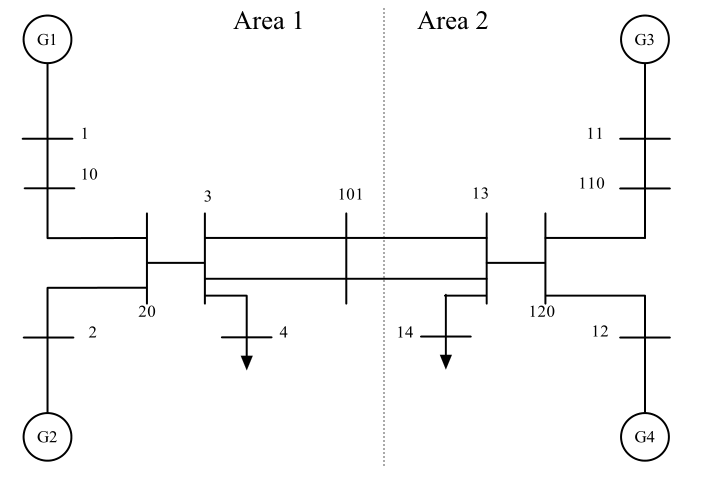
\includegraphics[width=\linewidth]{../200806-ExtendedVersionComp/sysOneLineAreas}
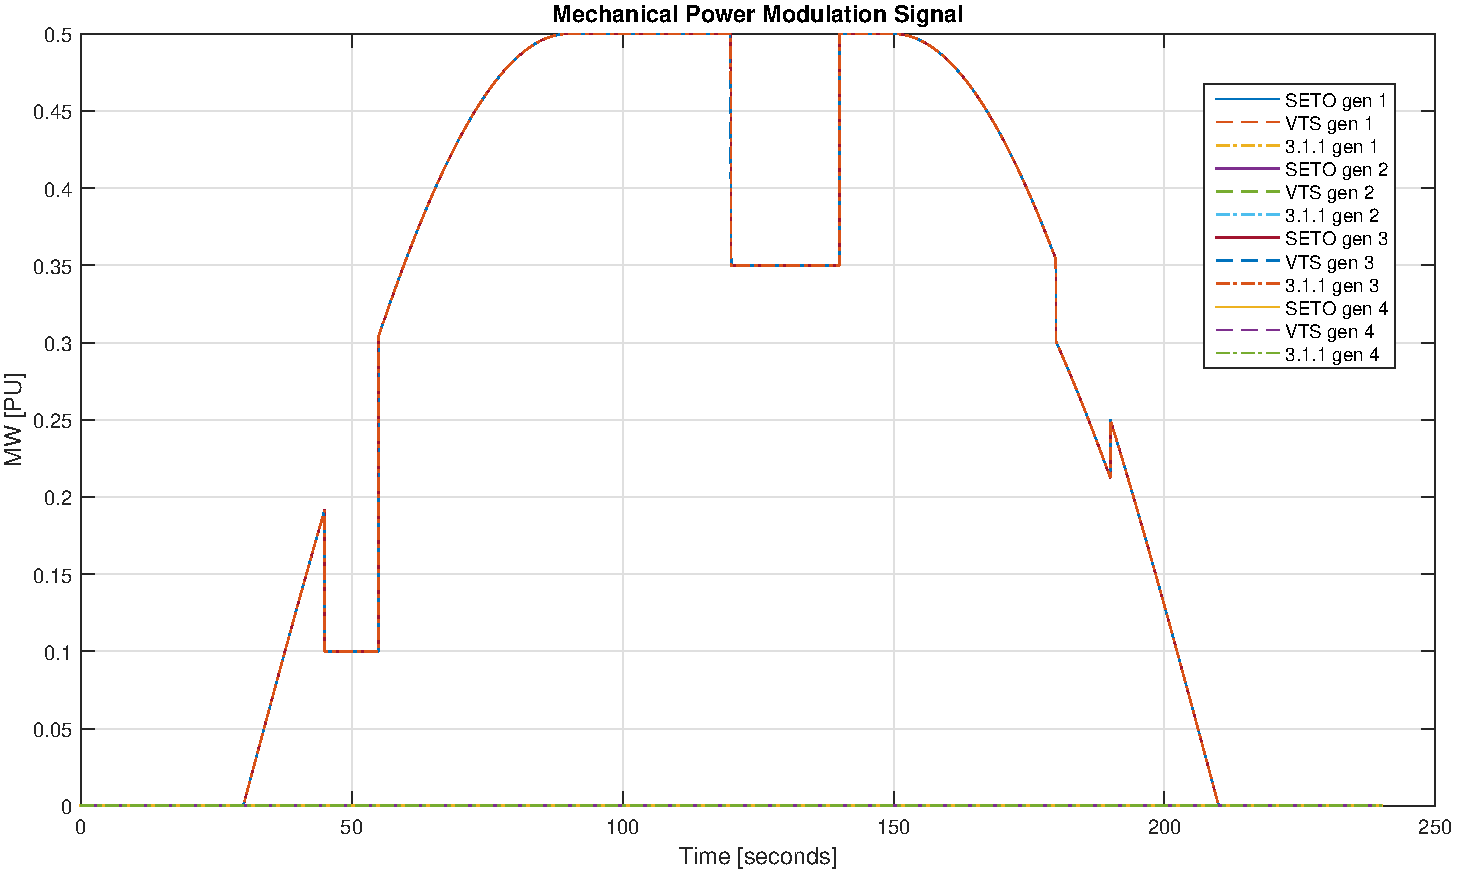
\includegraphics[width=.8\linewidth]{../200806-ExtendedVersionComp/verPmSig}
\end{minipage} %
\begin{minipage}{.47\linewidth}
\begin{itemize}
\footnotesize
\itemsep 0em
\item Kundur  4 machine system packaged with PST
\item Constant Z load model
\item System has governors, exciters, and PSS.
\item Governor of generator being perturbed by pm\_sig removed
\item Perturbance was meant to mimic a solar ramp with various situations of cloud cover:
\begin{Verbatim}[fontsize=\scriptsize]
% time [seconds]
% 0-30      - no action
% 30-90     - ramp up 0.5 PU (50 MW)
% 90-150    - hold peak
% 150-210   - ramp down 0.5 PU (50 MW)
% 210-240   - no action

% cloud cover events
% 45-55   - 20% max gen (generation of 0.1 PU)
% 120-140 - 30% cover (generation reduction to 70%)
% 180-190 - 15% cover (generation reduction to 85%)
\end{Verbatim}
\end{itemize}
\end{minipage}

\end{center}

\paragraph{Summary} 
\begin{enumerate}
\item Delay in executing pm\_sig caused by VTS created a noticeable delay in VTS dynamics.
\item Decreasing ODE solver tolerances did not resolve the issue.
\item Creating a new time block near the event in question did resolve the issue.
\end{enumerate}
As shown below, VTS may result with event start times ending up between computed time steps without additional user action/foresight.\\
\begin{center}
\centering
\begin{minipage}{.3\linewidth}
\centering
VTS 0
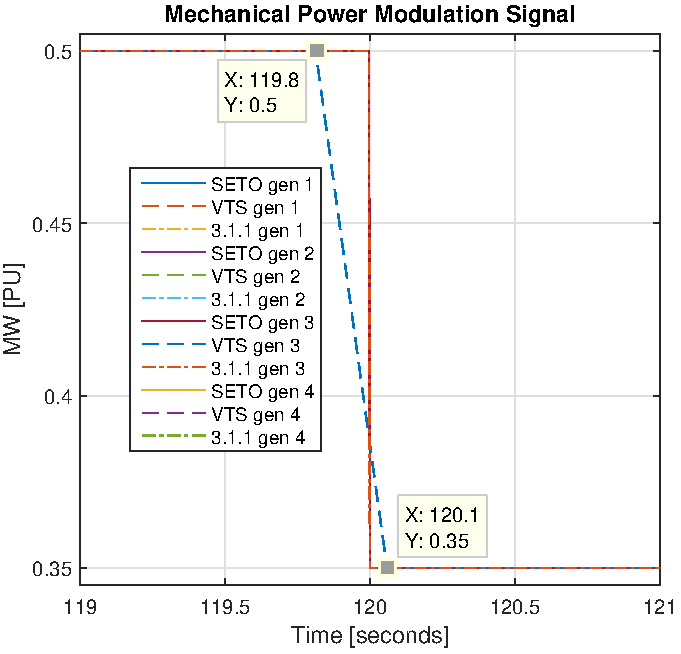
\includegraphics[width=\linewidth]{pmSig_0}
Original Simulation
\end{minipage} %
\begin{minipage}{.3\linewidth}
\centering
VTS 1
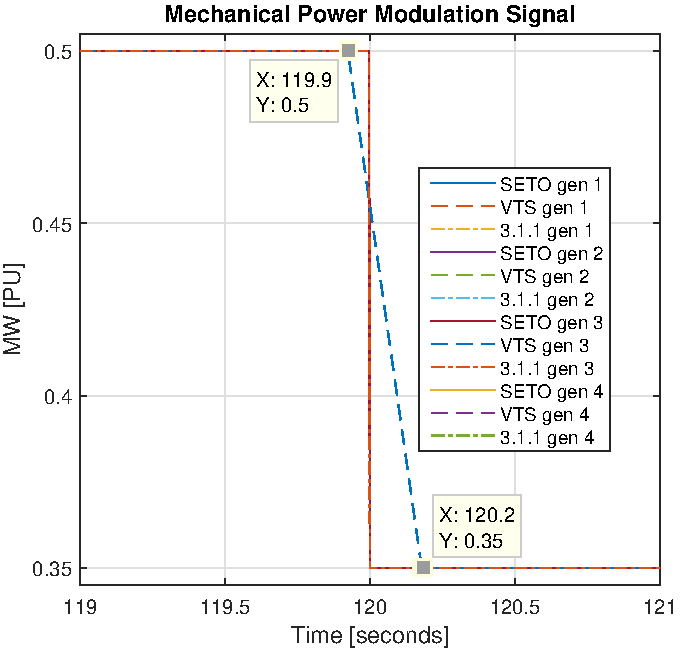
\includegraphics[width=\linewidth]{pmSig_1}
Decreased Tolerance 
\end{minipage} %
\begin{minipage}{.3\linewidth}
\centering
VTS 2
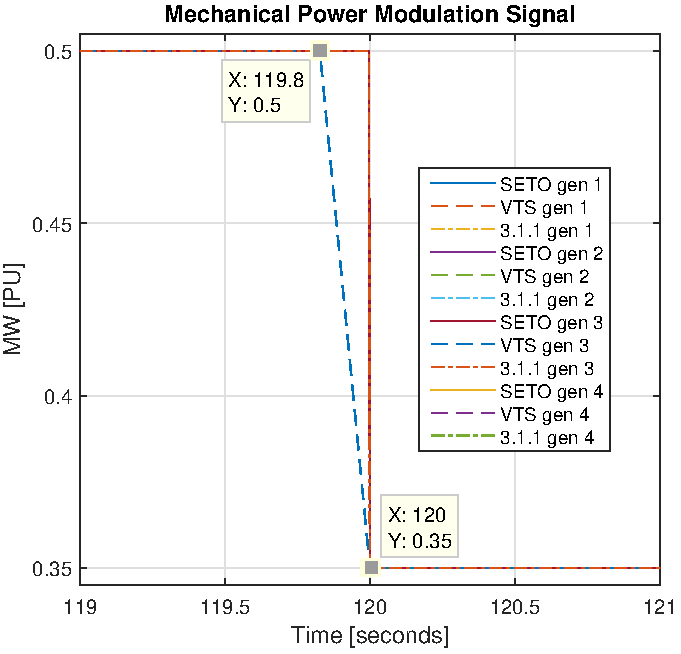
\includegraphics[width=\linewidth]{pmSig_2}
Additional `time block'
\end{minipage}
\end{center}
\pagebreak
\paragraph{sw\_con Changes} \ \\
The original switching array is shown below.
\begin{minted}[
		frame=lines,
		framesep=2mm,
		baselinestretch=1.2,
		bgcolor=gray!13,
		fontsize=\footnotesize,
	%	linenos,
		breaklines
				]{MATLAB}
ts = 0.004;
sw_con = [...
.1      0  	0  	0    0    0    ts;   % sets intitial time step
0.2     101	3  	0    0    6    ts;   % Do Nothing
30.0    0  	0 	 0    0    0    ts;   % Do Nothing
240.0   0  	0	  0    0    0    0];   % end simulation
\end{minted}
The altered switching array adds a null event at t = 120 to ensure the pm\_sig step is processed at the designed starting time.

\begin{minted}[
		frame=lines,
		framesep=2mm,
		baselinestretch=1.2,
		bgcolor=gray!13,
		fontsize=\footnotesize,
	%	linenos,
		breaklines
				]{MATLAB}
ts = 0.004;
sw_con = [...
.1      0  	0  	0    0    0    ts;   % sets intitial time step
0.2     101	3  	0    0    6    ts;   % Do Nothing
30.0    0  	0 	 0    0    0    ts;   % Do Nothing
120.0   0  	0 	 0    0    0    ts;   % Do Nothing <- Added row
240.0   0  	0	  0    0    0    0];   % end simulation
\end{minted}


NOTE: The start time of 0.1 was an oversight during case creation.


\paragraph{Performance Effects} \ \\ 
The decreased tolerance case (VTS 1 - with Relative Tolerance of 1e-5 instead of 1e-4) took more time to simulate as it took many more steps.
VTS 2, with the altered sw\_con, performed slightly slower than the original (VTS 0).
\begin{table}[!ht]
\resizebox{\linewidth}{!}{

	\begin{tabular}{@{} L{1.75cm} 
	R{2cm} R{2cm}  R{2cm} R{1.5cm} R{0.75cm} R{0.75cm} R{1.5cm} R{2cm} R{2cm}@{}} 	
		\toprule % @ signs to remove extra L R space
		\footnotesize % this will affect the table font (makse it 10pt)
		\raggedright % for non justified table text

	&	\multicolumn{3}{c}{Step Size [seconds]}					&		&	\multicolumn{2}{c}{Solutions Per Step}			&		&		&		\\	
Version	&	Max.	&	Min.	&	Ave.	&	Total Steps	&	Ave.	&	Max.	&	Total Slns.	&	Sim. Time	&	Speed Up	\\ \midrule	
VTS 0	&	2.32E+01	&	2.68E-04	&	2.58E-02	&	9,315	&	2	&	97	&	17,006	&	61.73	&	1.00	\\	
VTS 1	&	2.32E+01	&	1.36E-04	&	1.38E-02	&	17,353	&	2	&	96	&	27,243	&	106.09	&	0.58	\\	
VTS 2	&	2.00E+01	&	2.19E-05	&	2.58E-02	&	9,504	&	2	&	100	&	17,927	&	66.59	&	0.93	\\	
																				\bottomrule
	\end{tabular}
	}%end resize box
\end{table}

\pagebreak
\paragraph{Original Results (VTS 0)} \ \\

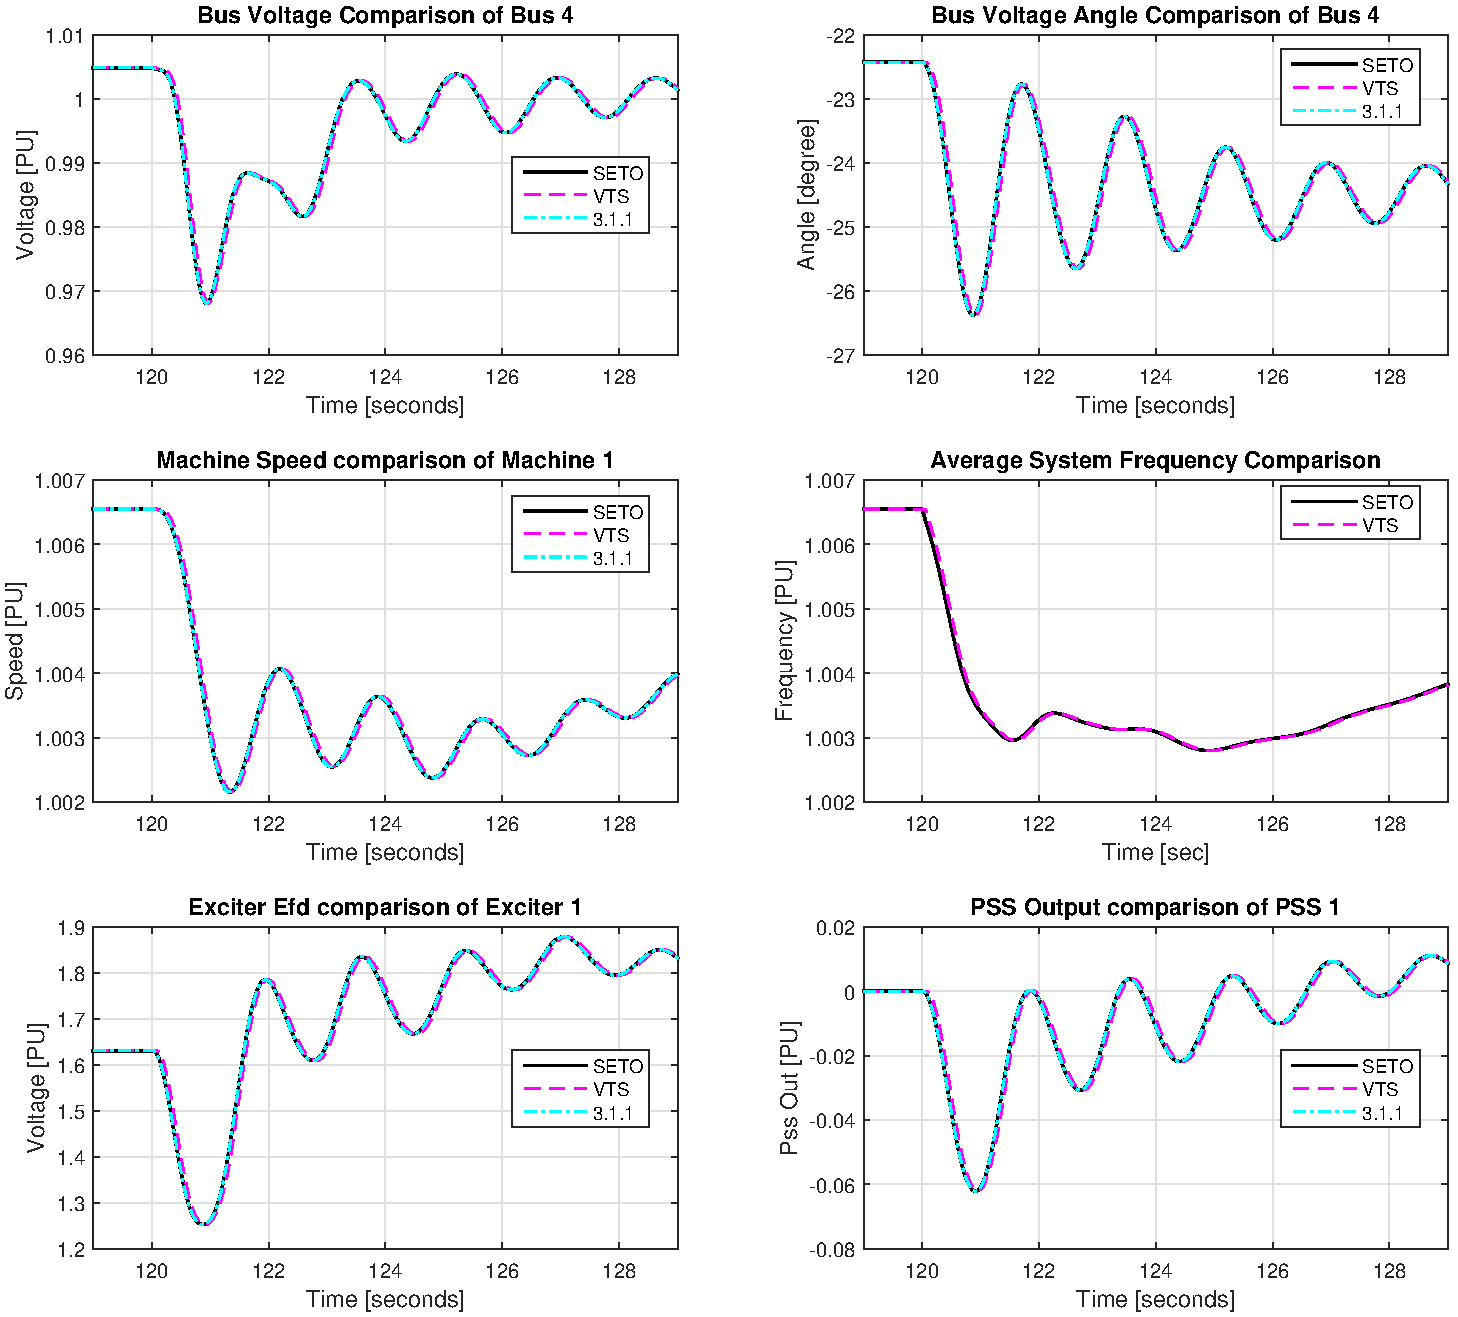
\includegraphics[width=\linewidth]{verCompDetail2}

\pagebreak
\paragraph{Decreased Tolerance Results (VTS 1)} \ \\

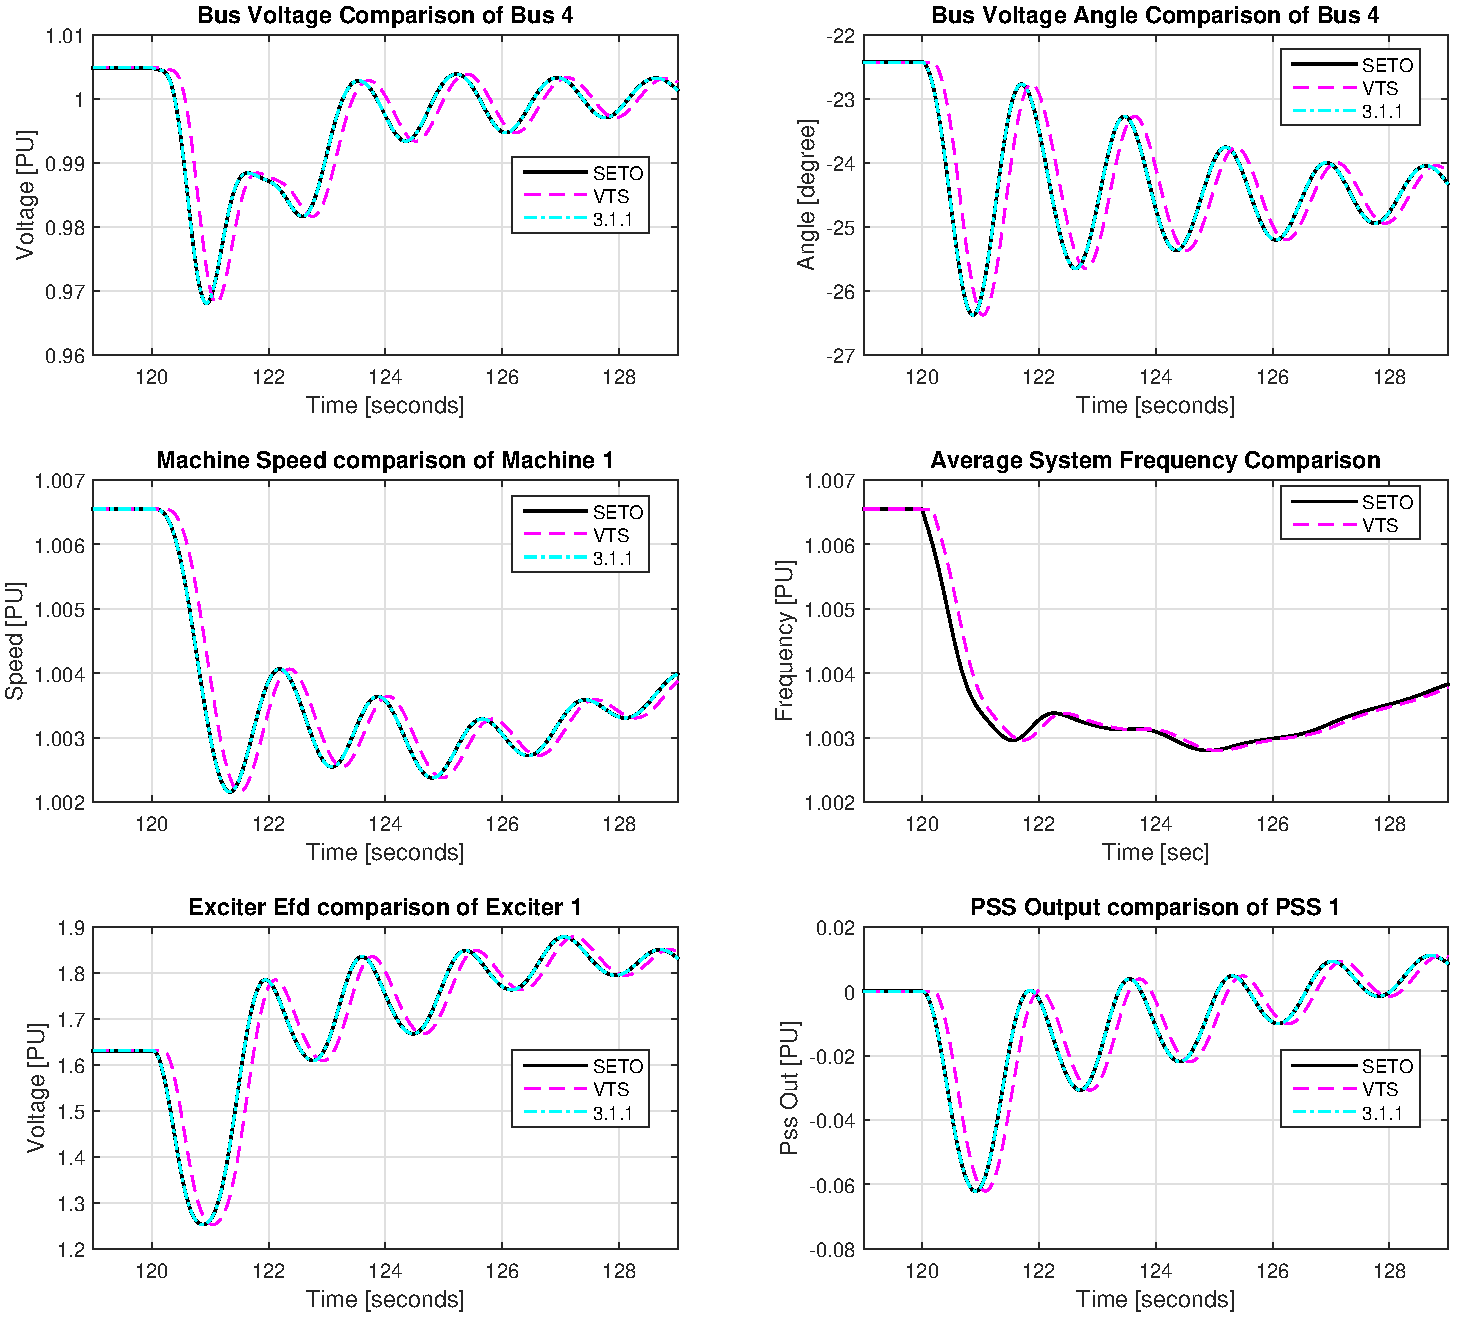
\includegraphics[width=\linewidth]{verCompDetail2ALT1}

Results actually appear worse than VTS 0 as there is more variance between expected and actual start time of the modulation signal.

\pagebreak
\paragraph{Altered sw\_con Results (VTS 2)} \ \\

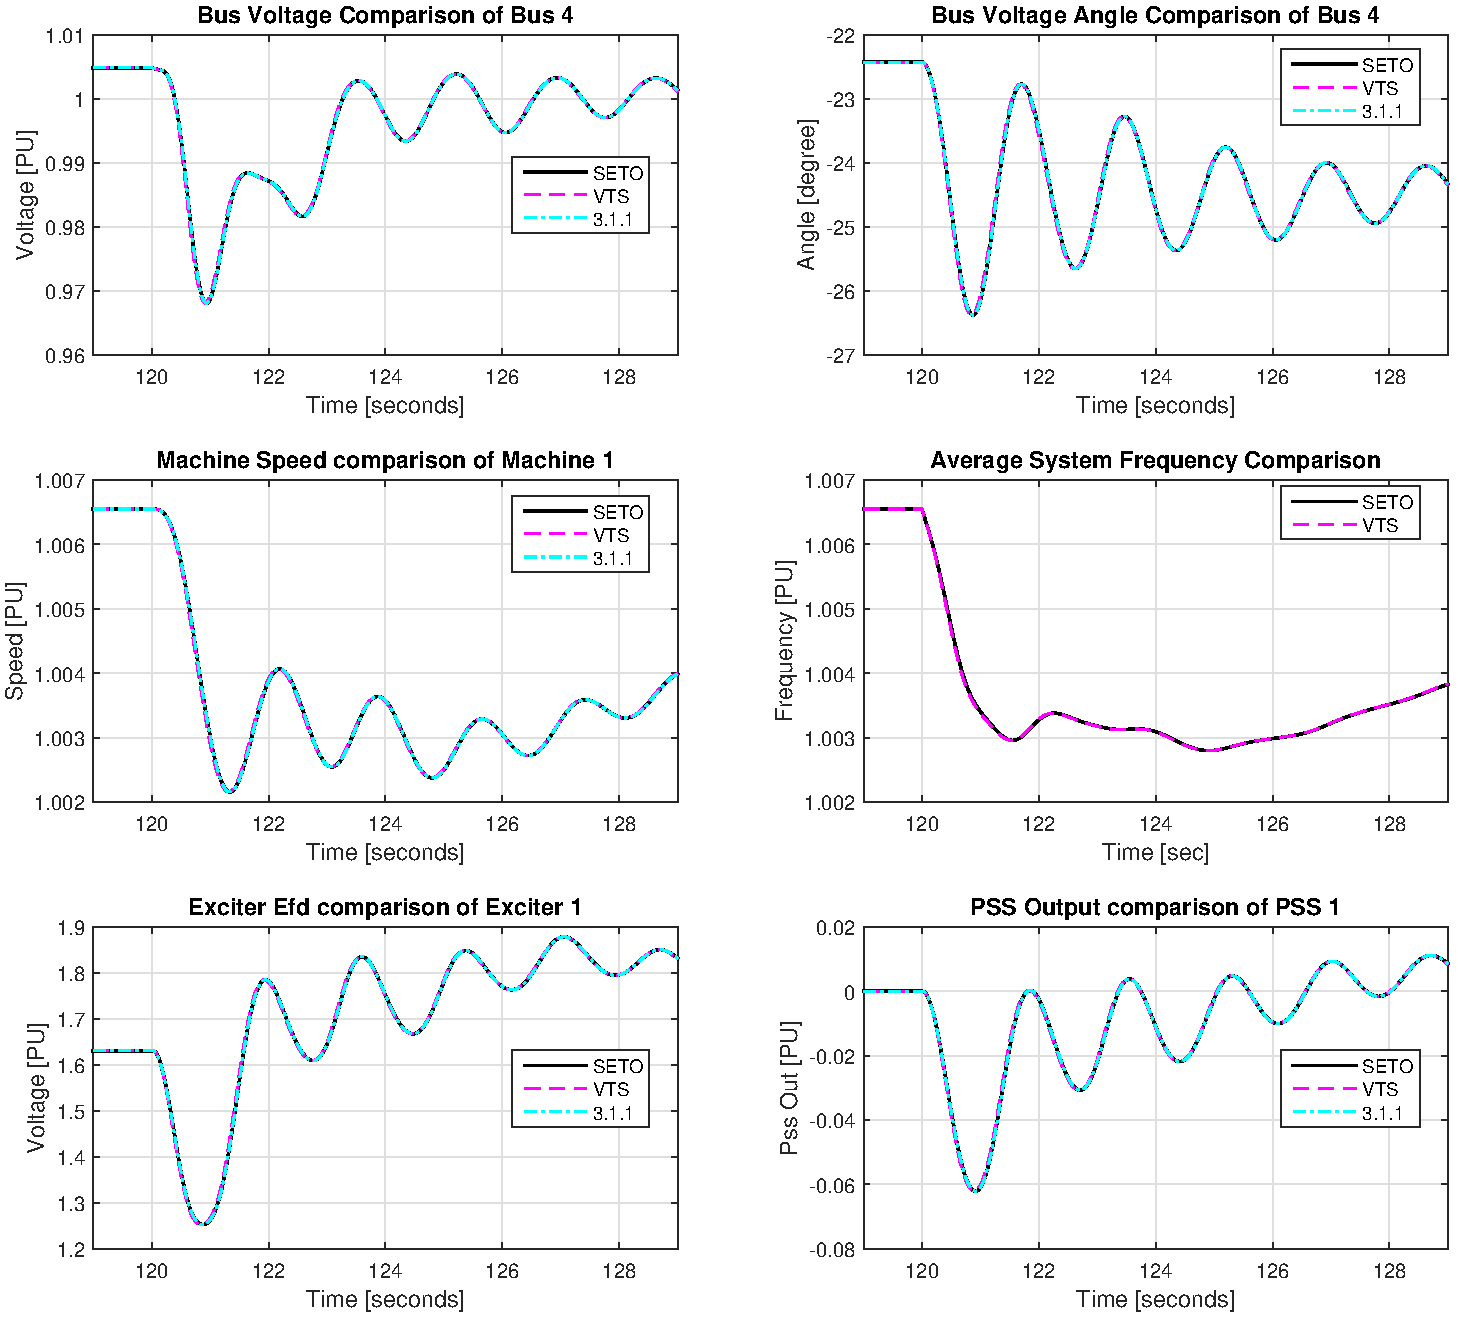
\includegraphics[width=\linewidth]{verCompDetail2ALT2}

The additional row in the switching control array seemed to resolve delayed dynamic issue.

\end{document}
